\documentclass[PPFS.tex]{template/subfiles}
\begin{document}
%--------------------------------------------------------------------------------
%	DESIGN CRITERIA, ALTERNATIVES, AND DECISIONS
%--------------------------------------------------------------------------------
\section{Design Criteria, Alternatives, and Decisions}

The design criteria, alternatives, and decisions for the project were divided into four parts based on the four main components of the gym reservation system. These four main components are the sensor system, the display interfaces, the hub, and the server.

\subsection{Sensor Systems}

The sensor systems constitute the means by which data is gathered from gym machines as to whether or not they are currently in use.

\subsubsection{Design Criteria}

The design criteria for the sensors used to gather machine usage information include a few characteristics. One criteria is that the sensors are capable of gathering movement data (like an accelerometer, gyroscope, or magnetometer) because each sensor will be mounted on a moving part of the machine. This data must be acquired reliably, which reflects the design norm of trust. Another criterion is that the sensors be relatively small (less than 5 in$^2$) so that they do not impede the use of the machine. Long battery life, on the order of years, is also a criterion for the sensors because it becomes inconvenient to replace the sensors for a whole gym. Through the sensors being small and having a long battery life, the design norm of delightful harmony will be incorporated. Additionally, a criterion is the ability of the sensors to operate in a mesh network, since this will decrease the amount of communication the hub has to do and will allow for shorter data transmission to and from each sensor. Lastly, the price of the sensor network must not be too high so that a gym owner could feasibly purchase it. By keeping the price within a reasonable range, the design norm of caring will be incorporated by considering the customer's needs.

\subsubsection{Design Alternatives}

The sensors chosen for the project must satisfy the design criteria set forth above. In researching different types of sensors, it became apparent that usually only two out of three desired characteristics exist in most sensors. These three main characteristics are the ability to use the sensors in a mesh network, the low cost of the sensors, and the ability to run on battery power for long periods of time. The final choice of sensors possessed all three characteristics, and is one of the main reasons these sensors were chosen for implementation in the design.

Much research has been conducted recently regarding sensors and sensor nets, but there are not many commercial products that are available. Research has been conducted at the University of California-Berkeley \cite{Berkeley_SmartDust, Berkeley_Nest} and the University of California-Los Angeles \cite{UCLA} regarding sensor systems and sensor networks. In addition, much research has been conducted at Stanford regarding the TinyOS operating system that runs on such sensor networks \cite{TinyOS}. All of this research has demonstrated the ability to construct a sensor network that operates reliably and at very low power, but few companies have advanced this research into a commercial product.

Despite the lack of commercial products, a few places do sell sensor networks. One of them is MEMSIC, which sells wireless sensor networks for a variety of applications, including educational, industrial monitoring, research and development, and location tracking. However, the boards that serve as wireless sensor nodes are a little expensive and are larger than desired for the project. \cite{Memsic}

Linear Technology is another company that sells wireless sensor networks. It provides nodes, or motes, at a low price that operate at very low power. However, these motes lack the sensors desired for the project, so additional sensors would need to be bought. \cite{LinearTech}

Developing or buying an Arduino board with the desired sensors is also an option, but the difficulty is found in finding an Arduino board that is capable of both mesh networking and sensor systems, is relatively cheap, and has long battery life. \cite{Arduino} There did not appear to be any public mesh networking libraries available for use that were built for Arduinos.

Bluetooth SensorBugs are also an option. They contain the desired sensors, are very small, and operate at low power. However, like many other sensors, they do not have the ability to form a mesh network, which is a key component of the project. \cite{Bluetooth}

Yet another option for wireless sensors is the CSRmesh development board. This board operates reliably within a wireless mesh network. However, it is expensive and does not include the sensors desired for the project (its main application is for lighting). \cite{CSRmesh}

Another option for sensors are TI SensorTags, which contain all of the desired sensors, operate reliably within a mesh network at low power, and are not too expensive. Because TI SensorTags satisfied all of the design criteria, they were chosen as the best design alternative. A more detailed description about this design alternative may be found in the section below. \cite{SensorTag}

\subsubsection{Design Decisions}

As seen in the previous section, each one of the design alternatives lacked one of the three main characteristics desired for the sensors with the exception of the TI SensorTags. As can be seen in \refFig{fig:TISensorTag1} and \refFig{fig:TISensorTag2}, the TI SensorTags possess the desired sensors in addition to many other sensors. These include a 9-axis motion sensor, a temperature sensor, a humidity sensor, an altimeter/pressure sensor, and an ambient light sensor. In addition, the TI SensorTags have the ability to communicate in a mesh network using Bluetooth, Zigbee, or 6LoWPAN. The battery lifetime for these sensors is about one year, and the data collection rate from the sensors can be modified as desired. In addition, the price per SensorTag is \$29, which is much lower than some of the other design alternatives. Because the TI SensorTags satisfied the criteria of having the desired sensors, operating reliably in a mesh network at low power, and having a lower cost, they are chosen to be implemented in the design. Each of the other design alternatives lacks one of the desired design criteria, as demonstrated in the decision matrix in \textbf{Table \ref{tab:sensorsMatrix}}. \cite{SensorTag}

% I will fill this in in a little while
\begin{table}[H]
   	\begin{center}
   		\caption{Sensor Systems Decision Matrix}
   		\label{tab:sensorsMatrix}
   		\begin{tabular}{|c|c|c|c|c|c|c|c|}
   			\hline
   			Design Factors & Weight & MEMSIC & Linear Tech & Arduino & SensorBugs & CSR Mesh & SensorTag \\
   			\hline
   			Movement Sensor & 9 & 8 & 0 & 8 & 9 & 0 & 10 \\
   			\hline
   			Small Size & 8 & 5 & 7 & 6 & 10 & 7 & 9 \\
   			\hline
   			Long Battery Life & 8 & 10 & 10 & 5 & 9 & 8 & 8 \\
   			\hline
   			Mesh Networking & 7 & 10 & 10 & 1 & 0 & 9 & 8 \\
   			\hline
   			Low Price & 6 & 6 & 7 & 8 & 7 & 4 & 7 \\
   			\hline
   			\textbf{Total} & & 298 & 248 & 215 & 275 & 207 & 324 \\
   			\hline
   		\end{tabular}
   	\end{center}
\end{table}

\begin{figure}[H]
	\centering
	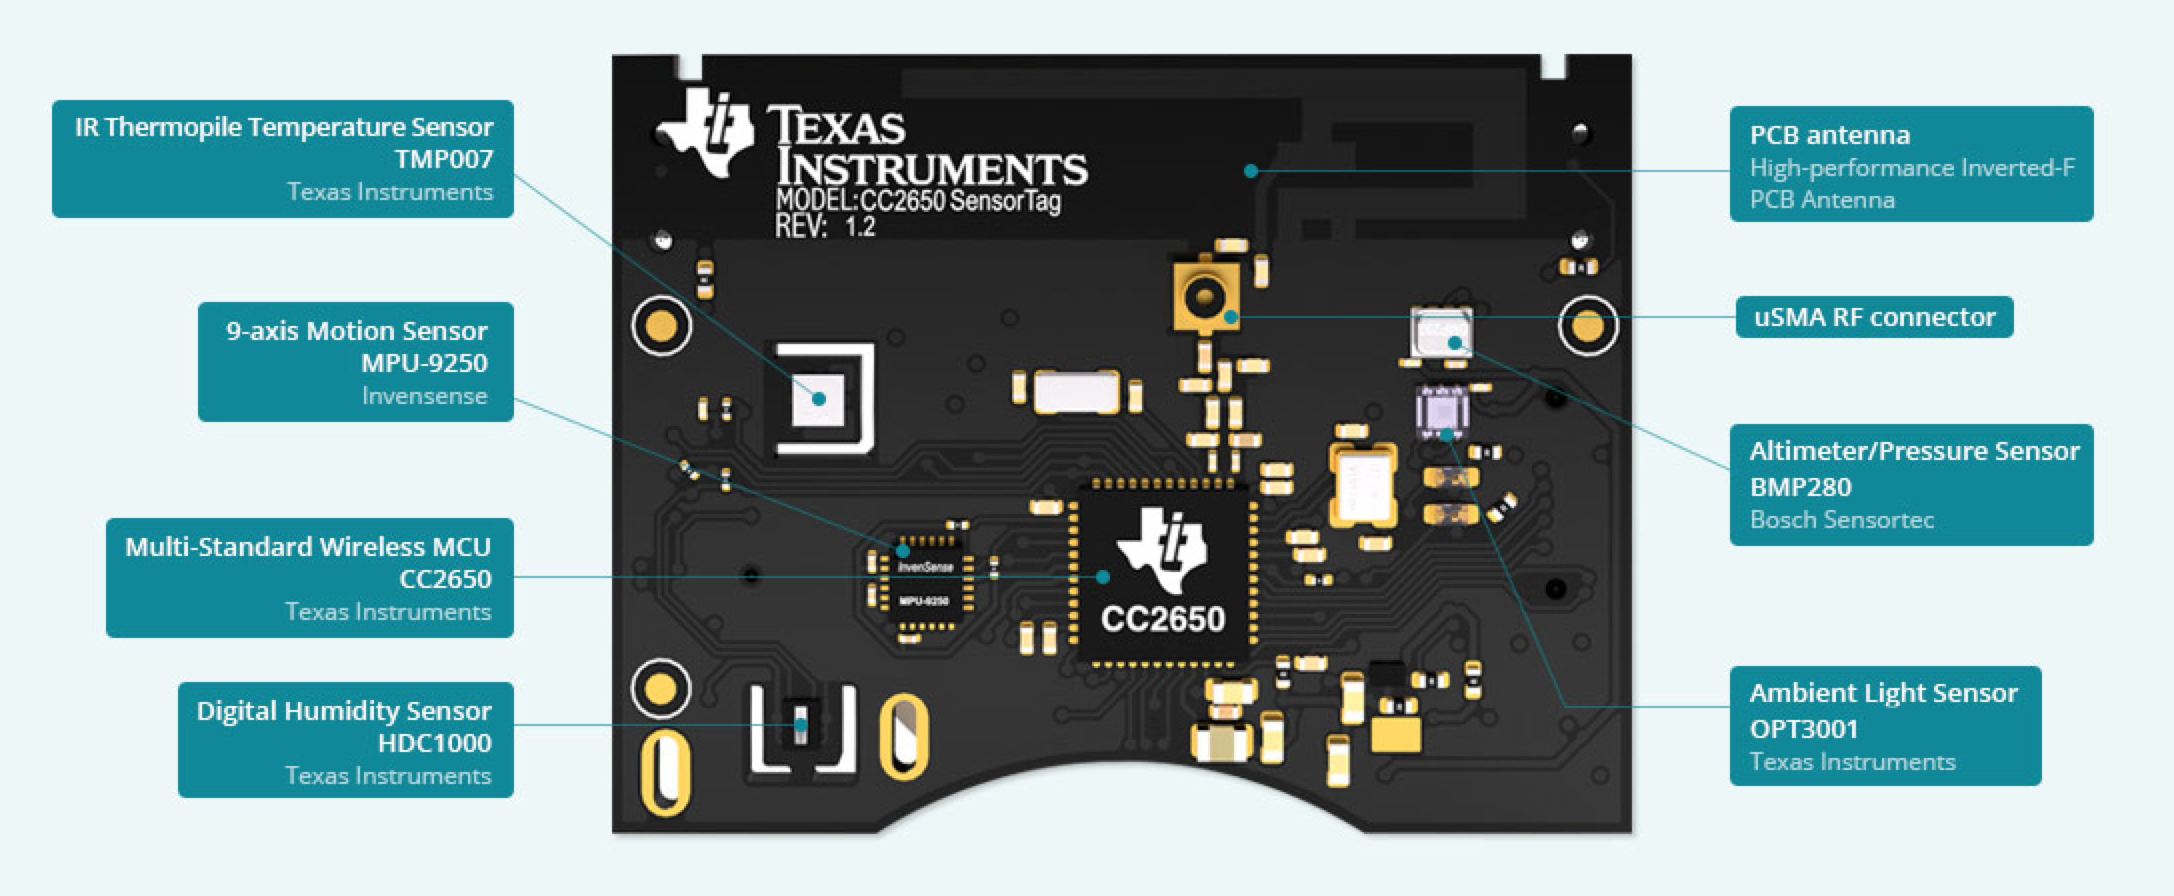
\includegraphics[width=0.9\textwidth]{SensorTag/SensorTag_1}
	\caption{TI SensorTag Sensors and Microcontroller}
	\label{fig:TISensorTag1}
\end{figure}

\begin{figure}[H]
	\centering
	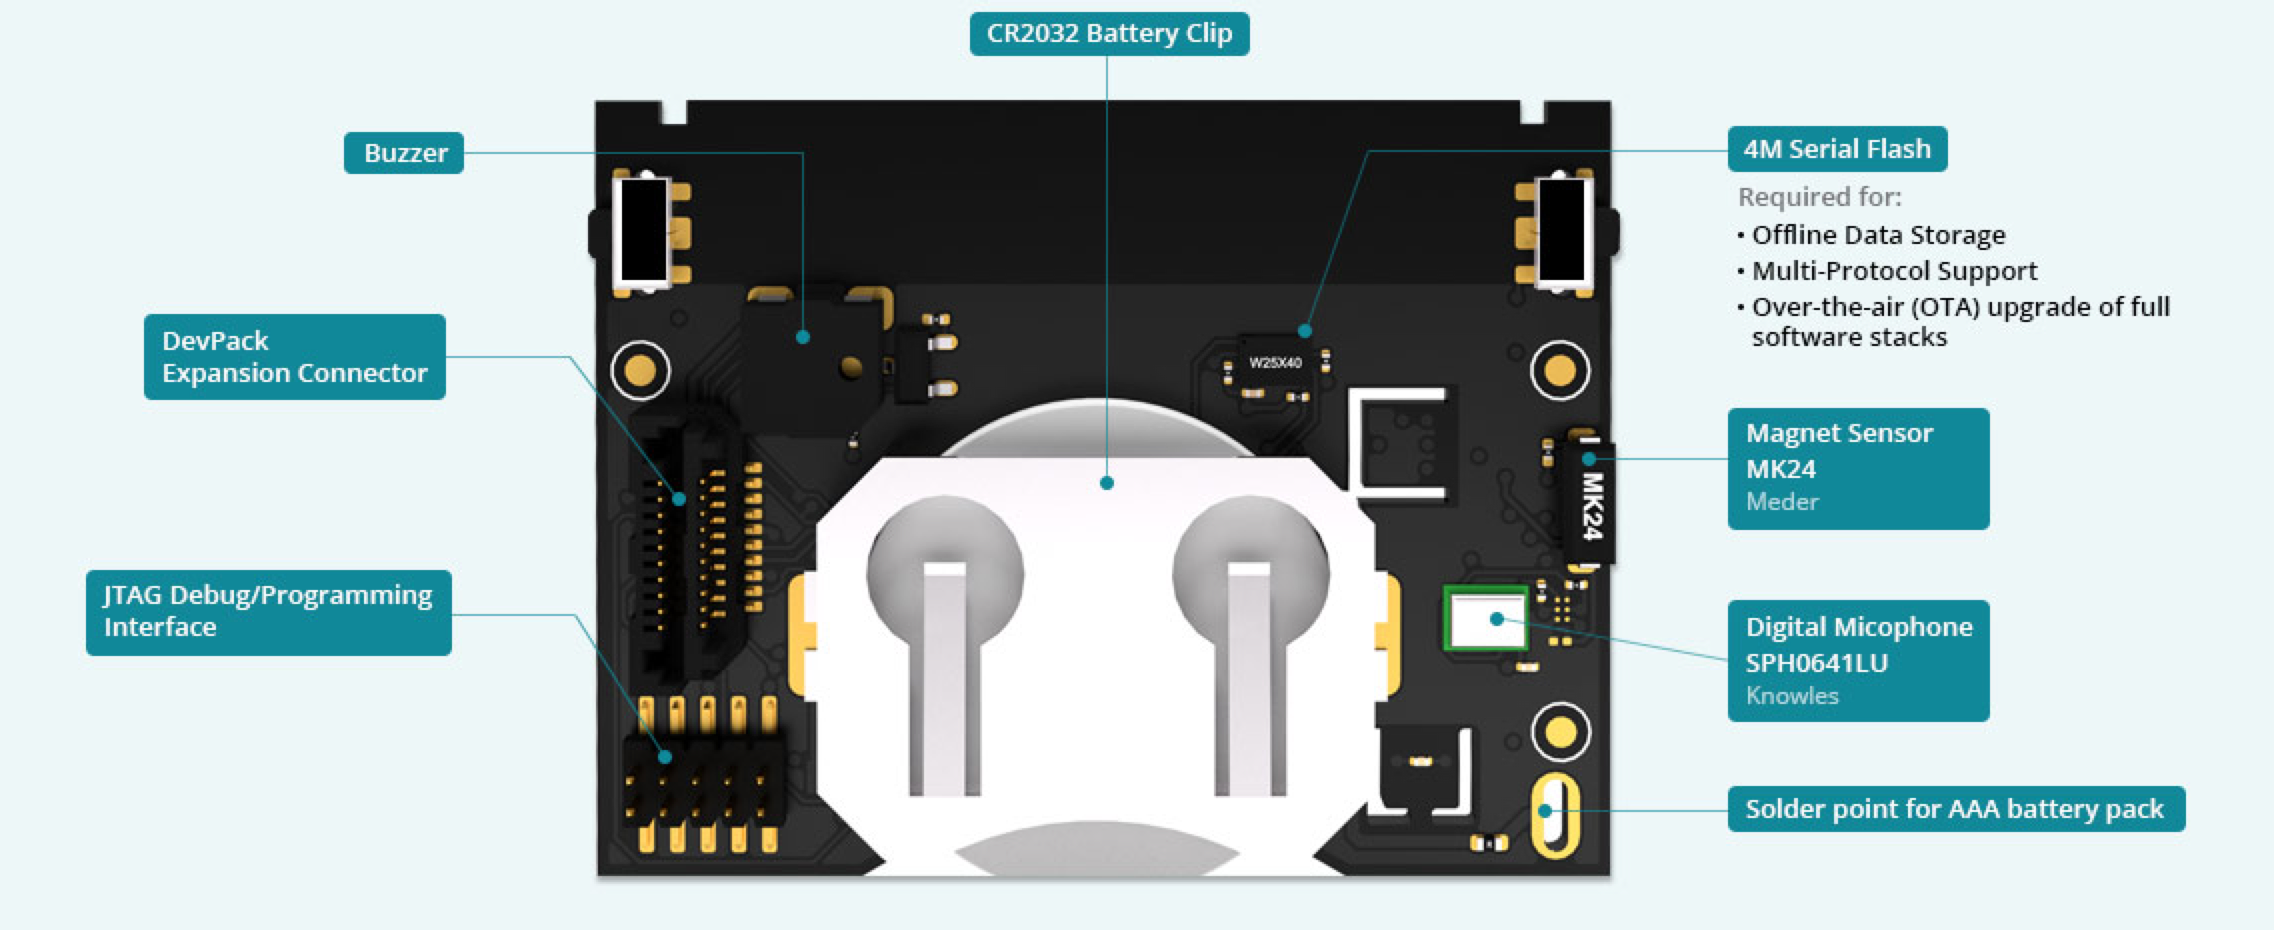
\includegraphics[width=0.9\textwidth]{SensorTag/SensorTag_2}
	\caption{TI SensorTag Sensors and Connections}
	\label{fig:TISensorTag2}
\end{figure}

% Dan
\subsection{Display Interfaces}

The display interface allows the user to see current reservation information for a machine.

\subsubsection{Design Criteria}

Multiple design criteria have been used to select the optimal display interface. Battery life is an important criterion as it reduces the time spent by gym managers replacing or recharging batteries.

The range of a display interface and its ability to connect in a mesh network are also design criteria as they affect how large of a gym in which the system can be installed.

Simplicity is a third criterion as smaller or simpler boards are less obtrusive, promoting delightful harmony. In order to make the transition from a prototype to a real product, boards with available and open source hardware design files are preferred.

Lastly, the display interface constitutes a large portion of the cost of the system. Any variation in the cost in a single unit is multiplied since many display interfaces are purchased for one system. Thus cost is an important design criterion.

\subsubsection{Design Alternatives}

As a result of these criteria, four devices have been chosen as alternatives for small low-cost boards that could fulfill the design requirements: a Raspberry Pi, an Arduino, a CC3200 Launchpad, and a TI SensorTag. 

For the display component of the display interface, the applicable criteria are battery life and price. Due to the fact that the board needs to run on batteries, the display cannot require a significant amount of power. This negates most typical Liquid Crystal Display (LCD) options. The two low power options that were found are E-Ink (also known as E-Paper) and Memory LCD. E-Ink has the advantage of requiring no power when the image is not changing, which would be most of time in this project. Memory LCD, on the other hand, does require some power, but typically under \SI{200}{\micro\watt}, which means a single AA battery would last over 200 days. The original target display size was 2" x 3"; however, the closest available size for either type of display is 2.7" (35mm x 59mm) with similar prices. Each of the four board alternatives can support at least one of these display options.

The Raspberry Pi (shown in \refFig{fig:raspberryPi}) is a credit card sized computer that runs a full Operating System (OS), such as Linux or Windows 10, with Universal Serial Bus (USB) ports and a High-Definition Multimedia Interface (HDMI) output. Most importantly, it has 40 General Purpose Input/Output (GPIO) pins that can be used to connect the display or other features like buttons and a wireless communication device.

The advantage of this board is that it has the most community developed libraries, including already built libraries for mesh networking and for controlling E-Ink displays, which would make the display interface very easy to build. Breakout boards for E-Ink displays are available for the Raspberry Pi and are well priced, which would make adding the display simpler. This board is also inexpensive; a \$20 model would easily fit the requirements.

However, the Raspberry Pi has much more functionality than needed. Combined with fact that it is running an OS, it uses much more power than any of the other options, making it virtually impossible to run off battery. There are some batteries that might work for a few days, but they are expensive and rather large for this board. Along with the fact that it is not an open source board, the complexity of the Raspberry Pi would make it hard to use as an actual product. The price of a display interface with this board would likely be about \$90.

\begin{figure}[h]
	\centering
	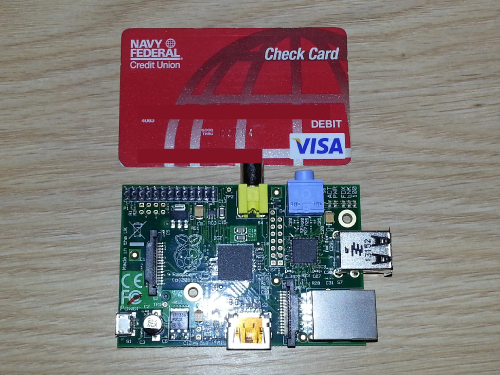
\includegraphics[scale=0.5]{RaspberryPi.png}
	\caption{The Raspberry PI, a Credit Card Sized Single Board Computer}
	\label{fig:raspberryPi}
\end{figure}

The Arduino is an open-source prototyping board that runs a single program. It also has GPIO pins for controlling the display and connecting a wireless communication device.

Some basic Arduino boards are quite low priced, and there is also a big community behind Arduino boards. The fact that an Arduino runs only a single program can make it very power efficient, thus making operating it by battery over several months plausible, even using AA batteries. There is at least one reasonably priced E-Paper breakout board that eases the process of adding a display.

The only mesh network library found was for a radio frequency (RF) radio, though that may not be a disadvantage as it may be more power efficient than some other solution. Also, a lot of libraries use code that does not take power efficiency into account, which limits either the battery life or the libraries available. The price of a display interface with this board would likely be about \$60.

The CC3200 chip is a microcontroller with built-in Wi-Fi. The CC3200 Launchpad is a board designed to provide features for this chip such as GPIO pins, USB interface, and power.

The primary selling point of this chip is the built-in Wi-Fi which translates to good power efficiency, allowing the board to run very well on batteries. An E-Ink breakout board is available and has available design files. Along with the fact that the design files for the Launchpad are easily accessible, this board would be the easiest to transition from a prototype device to a commercial one. An additional advantage is that the built-in Wi-Fi is FCC approved, unlike many add-on Wi-Fi dongles, which removed a roadblock to commercialization.

However, no mesh network library could be found for the CC3200. The E-Ink breakout board for the CC3200 Launchpad is also quite expensive and large. The price of a display interface with this board would likely be about \$80.

The TI SensorTag is a small board made for prototyping IoT devices and is shown in \refFig{fig:TISensorTag1} and \refFig{fig:TISensorTag2}. This board has a built-in communication device that supports ZigBee, a protocol design for mesh networking, and is made to last extended periods of time on a coin cell battery. It also has a devpack for a "smart watch," which acts as a breakout board for memory LCD displays. The board has open hardware and software files which would facilitate the transition to a commercial product. Since the SensorTag was chosen as the sensor for the system, selecting it would result in only having to use one type of board for both the sensor and the display interface, thus streamlining the system. This might also eliminate the need for a separate sensor, which would reduce cost significantly.

However, the devpack comes with various accessories including a 1.3" memory LCD, while the only desired component is the connector for the memory LCD. The larger memory LCD display would need to be bought separately. The price of a display interface with this board would likely be about \$70. This cost could be further reduced if the breakout board for the memory LCD display could be replicated so that the smartwatch devpack would not need to be bought for each display interface.

\subsubsection{Design Decisions}

While overall the Raspberry Pi is a good board, the difficulty and price of running it by battery and its complexity mean that it has not been chosen for the system. This would be a good solution if the project allowed for a power supply instead of batteries. The Arduino is a good option since it is the least costly and fits all the requirements fairly well, making it the second best choice. The CC3200 Launchpad would be the easiest choice in transitioning to an actual product, but it would be the most difficult to use in getting a prototype working. Along with the cost, this solution was not chosen for the project. While the price of the SensorTag may not be as low as the Arduino, the battery life and the built-in mesh networking are huge advantages. The fact that this board can also be used for sensors and is open source make this the top candidate for the project, as shown by the decision matrix in \textbf{Table \ref{tab:displayMatrix}}.

\begin{table}[H]
   	\begin{center}
   		\caption{Decision Matrix for the Display Interface}
   		\label{tab:displayMatrix}
   		\begin{tabular}{|c|c|c|c|c|c|}
   			\hline
   			Design Factors & Weight & Raspberry Pi & Arduino & CC3200 Launchpad & SensorTag \\
   			\hline
   			Battery Life & 10 & 2 & 7 & 7 & 10 \\
   			\hline
   			Network Capabilities & 5 & 8 & 7 & 3 & 10\\
   			\hline
   			Simplicity & 2 & 8 & 10 & 1 & 10 \\
   			\hline
   			Open Hardware & 3 & 8 & 8 & 5 & 9 \\
   			\hline
   			Cost & 10 & 11 & 17 & 12 & 14 \\
   			\hline
   			\textbf{Total} && 201 & 321 & 245 & 338 \\
   			\hline
   		\end{tabular}
   	\end{center}
\end{table}

% Ryan
\subsection{Hub}
The Hub is the component through which the data from the display and sensor networks is passed to the server and from the server out to the displays. It is essentially the gateway for the system between the gym and the Server.

\subsubsection{Design Criteria}
The most important aspect of the Hub is its ability to communicate. Since it can be hidden and plugged in, form factor and battery power are not necessary considerations. This opens up options to using full small computers as long as they have the ability to communicate with the sensors and displays, along with the computing power necessary to serve as the client to the server. In order to minimize the cost of the system, the board needs to be cheap but still have the necessary computing power. For the communication to be as reliable as possible an Ethernet port is necessary on the Hub.

The design norms that can be applied to the Hub component are transparency and trust. Transparency is shown by being open and forward with the gym administrators as to what information the Hub is passing onto the server and how it uses the gym's existing Internet for that proces. Trust is applied through the security of the software and the encryption of the data that is passed back and forth between the Hub and the Server. Ensuring that the user's data is secure is important in order for users to feel safe in continuing to use the system.

\subsubsection{Design Alternatives}
The primary options for the hub were different models of the Raspberry Pi, the Intel Edison board, or possibly some other single board computer. There is an increasing number of single board computers available on the market, and they are getting cheaper and faster. In considering these various boards, one large difference is the size of the community using the boards and the number of devices available that can easily interface with them. Most of the boards would have worked well for this application, as the necessary network communication can be connected via a USB port and the software needed to collect the Zigbee data can run on Linux. Due to the fact that this component can be plugged into permanent power, this opens up the possibility of any computer device running Linux and having a USB port as being a viable option. The reasons for narrowing this field down to simply the Pis and the Edison board is due to their large support, stability, and their low price point.

The Edison board has the advantage of having lower power consumption and the support of a large company. However, it does not have an Ethernet port and is approximately double the price of a Pi, as can be seen in \textbf{Table \ref{tab:hubMatrix}}. The Edison board is also intended as more of a sensor board than a small computer, though it could work for this project with the right breakout boards. \cite{Intel}

There are multiple models of the Raspberry Pi boards, each one with improved specs over the previous model, generally in the form of more Random Access Memory (RAM), a faster Central Processing Unit (CPU) and Graphics Processing Unit (GPU), and additional ports. The main difference with the most recent Pi, as compared to previous ones, is its ability to run Windows 10. This is not currently a requirement of this project, though. However, if the sensor's software is made for only Windows, it could be a potentially useful aspect of choosing the newest Pi, the Raspberry Pi 2 Model B. The older versions of the Raspberry Pi should be adequate for this project, though. As long as there is no need for Windows 10, then the computational power differences should not make an impact on this project. For the amount of computing power that Pis provide they are the cheapest single board computer currently available on the market. This is due to their success and large scale production. An additional advantage of this large scale is that Pis have a stable Linux Operating System (OS) developed specifically for them, which should help minimize any bugs in the system and increase the stability. \cite{RaspberryPi}

The other aspect of the hub to be considered besides the single board computer is how it will communicate with the sensor and display network. The only connectivity built into the Raspberry Pi is an Ethernet port. This means that whatever wireless technology is used will need to be added through either the GPIO pins or a USB dongle. There are options for Bluetooth dongles \cite{AdaFruit}, Wi-Fi dongles \cite{RaspberryPi}, and Zigbee modules \cite{Zigbee} that a Pi can use. All of these options enable the Pis to connect to whichever network ends up being used. This is one area were the Edison board has an advantage, as it has Wi-Fi and Bluetooth connectivity built into the main chip and is primarily designed as an IoT board \cite{Intel}. However, since reliability is an important factor, the inclusion of an Ethernet port on the Pis is more important than the Edison Board's capability with Wi-Fi and Bluetooth. This is especially true since the network technology may be something besides Wi-Fi or Bluetooth, which would require an additional dongle to any chosen board, such as Zigbee or 6LoWPAN.

\subsubsection{Design Decisions}
The final board that was chosen was the Raspberry Pi 2 Model B. This board was chosen because for its price it had the most options. Primarily, it was chosen to accomadate for potential future design changes, like running Windows 10 on it. This board is available for \$35, has more than the needed requirements, and can use the Zigbee module via the GPIO pins as opposed to the USB through a breakout board, saving some money. However, the board that is currently being used as a prototype is a Raspberry Pi Model B+. This is because Calvin already had several older Pi models available for use and the small advantage that the Pi 2 would offer is not necessary unless for some future design change Windows 10 becomes necessary. This change from the initial design decision saved some money in the budget and enables the team, if necessary, to purchase an additional sensor or display later in the project. There is also enough money in the budget if the purchase of a different single board computer becomes necessary.

       \begin{table}[h!]
       	\begin{center}
       		\caption{Decision Matrix for Hub Hardware}
       		\label{tab:hubMatrix}
       		\begin{tabular}{|c|c|c|c|c|}
       			\hline
       			Price && \$40 & \$95 & \$35 \\
       			\hline
       			Design Factors & Weight & Pi 2 Model B & Edison Board & Pi 1 Model B+ \\
       			\hline
       			Network Capabilities & 10 & 5 & 5 & 5\\
       			\hline
       			Ethernet & 8 & 10 & 1 & 10 \\
       			\hline
       			Range & 8 & 5 & 5 & 5 \\
       			\hline
       			Costs & 5 & 8 & 1 & 9 \\
       			\hline
       			Reliability & 10 & 10 & 10 & 9 \\
       			\hline
       			\textbf{Total} && 310 & 203 & 305 \\
       			\hline
       		\end{tabular}
       	\end{center}
       \end{table}

% TJ
\subsection{Server}
The server will handle all connections requesting information about the current status of the machines, along with making and viewing reservations for the equipment. It will also handle sending historical data for administrators and personal historical data for individual users. It takes all the data from the server and stores it, creating these services for the client.

\subsubsection{Design Criteria}
The server's primary requirement was that it must be reliable. Both the gym administrators and the gym's clients must be able to trust that when attempting to ascertain information about the machines, whether historical or current information, that the information can be sent to them. The server must be capable of modern networking protocols and functions, including HTTP/HTTPS requests and creating and maintaining TCP network connections. The HTTP requests requirement is to enable the server to send information about the state of the machines over the internet to clients of the system. The TCP network connections are to ensure a reliable connection between the hub and the server for consistent and reliable information sharing. The server must also be powerful enough to encrypt data and send data over encrypted connections to make sure that all client information is protected.

\subsubsection{Design Alternatives}
There are in essence two main players in the server world: Windows and Linux. Both of these options have the capabilities to meet the requirements stated above in the Design Criteria section, however Linux has several advantages. The first is that it is free, which will reduce the cost of our system. The second is that it is often more
% Need a citation here
reliable.

\subsubsection{Design Decisions}
It was chosen to use Ubuntu 14.04 as the server. It provides the reliability required to provide the users with a trustworthy experience. It also should be low maintenance once installed, as security and software updates can be handled automatically using built-in Linux functionality. Ubuntu 14.04 is the Long Term Supported (LTS) version of Linux currently and will be supported for
% Need exact date
several more years. It also has the modern capabilities to use Python and other libraries to create secure and consistent connection with the Hub. Also because the hub is running Linux, it makes sense to continue to use the same operating system for ease of upkeep. It also aligns with the teams goal of transparency because Linux is an Open Source solution to the problem the team is faced with.

\end{document}
